\chapter{Concept and Design}
\label{cha:conceptanddesign}

This chapter outlines the key components of the implementation of environments in the MS.
The core components are users, environments, roles, and assets.
In essence the concept can be summarized as follows: users can be part of multiple
environments, which hold Assets.
Users that are part of an environment can work on the assets that are stored in it.
Each environment has a set of permissions that determine what their users can do with its
assets.
All other components that will be introduced will help to manage and enforce these relationships.

\section{Modifications to Assets and Resources}

This thesis will modify the assets \ref{cha:relatedwork:proceed-assets} and the resources
\ref{cha:relatedwork:proceedroles:ms-resources-actions} that supported by the MS,
these will be modified to be contained inside environments.
Additionally, environments will be added to the MS' assets and resources.
As will be explained in \ref{cha:conceptanddesign:users}, Users won't belong to a single
environment, they can instead be members of multiple environments, for this reason,
users will be removed from the MS' assets and resources.
Furthermore, folders and  memberships will be added to the MS' assets and
resources.

\section{Users}
\label{cha:conceptanddesign:users}
%NOTE: maybe change the sctructure of this paragraph a bit

Previously all users in the MS were members of a single organization.
In order for users to be part of multiple organizations, they can't be tied to a single
organization.
As a part of the implementation of environments, users are now independent of
organizations,
they represent individual people utilizing PROCEED and will be stored as entries in
the MS' storage solution \ref{cha:ms-architecture:data-storage}.
% A single person can have one or more users, but each user is intended for individual use.

To facilitate the exploration of the MS, without creating a user, we introduce the option
to use the MS as a guest.
Thus, we differentiate between authenticated users and guest users.
Guest users have a limited feature.
Guest users can transition to being an authenticated users whilst retaining their
assets, to do this they will need to sign in with personal data.
% Creating a Guest user doesn't require any data from the person creating it.

All users have a personal environment \ref{cha:conceptanddesign:environments:personal}
in which they can create and manage assets freely.
Authenticated users can also be part of and create organization environments
\ref{cha:conceptanddesign:environments:organization},
where they can collaborate with other users.

\subsection{Authenticated Users and Accounts}

% NOTE: is Oauth2 account the correct term here?
To allow the same user to be able to sign in with different Oauth2 providers, e.g. with Google,
Facebook or Discord, we store a separate record, called account, for each of the user's sign-in methods.
% NOTE: should one to many be explained?
This means, that the relationship between users and accounts is one-to-many,
a user can have multiple accounts, but an account can only be linked to one user.
This way, when a user is signing in with credentials from an Oauth2 provider,
the MS can look up the corresponding account to the credentials, and then find the user
that the account is linked to.

\begin{figure}[H]
	\centering
	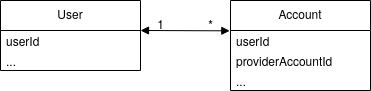
\includegraphics[scale=0.6]{images/users-accounts-relation.drawio.png}
	\caption{Relation between users and accounts.}
	\vspace{-1em} % Negative value to remove space
\end{figure}
% caption: Relationship between users and accounts.

\subsection{Merging a Guest User with an Authenticated User}
\label{cha:conceptanddesign:users:mergeguestuser}

As previously stated, a guest user can transition to being an authenticated user by
signing in with his personal data.
It could be the case that his personal data already corresponds to an existing user.
In this case, the user will be asked if he wants to merge his assets with the existing
authenticated user.
If he chooses to merge, all the assets in the guest user's personal environment will be
transferred to the authenticated user's personal environment.
Otherwise, all the assets created by the guest user will be deleted.

\subsection{Guest User Storage}

For storing guest user data, one could take one of two approaches:
storing the data in the user's browser or storing it in the MS' database, alongside the
data of authenticated users.
Storing the data locally has two great benefits:
The MS doesn't have to store data of users who might never return and
the MS would become less susceptible to an attack where the attacker tries to use up as
much space as possible in the MS' storage solution.
However, this approach has one key downside, the MS would have to implement two storage
solutions and the frontend would need to switch accordingly between them.
The added complexity would make it harder for developers to get an overview of the MS'
codebase and it also makes it harder to use coding assistance features of IDEs like Goto
definition \footnote{\url{https://microsoft.github.io/language-server-protocol/specifications/lsp/3.17/specification/\#textDocument_definition}}.
For this reason, storing guest user's data locally isn't worth the benefits.
So we decided to store a guest user's data in the MS the same way we do it for
authenticated users,
with the difference that a flag is set
% in the user entry to 
indicate that he is a guest.
This way, all the endpoints that authenticated users can call to interact with the MS
can also be called by guest users.
An important caveat is that, to enforce some of the feature restrictions, relevant
endpoints have to check whether the user is a guest.
Furthermore, the MS needs to clean up inactive guest users, to prevent the MS' storage
solution from filling up with unused data.

\subsection{Development Users}

When developing the MS, it is not common for the developer to have all the necessary keys
configured in the environment variables, for the MS to be able to authenticate users with
Oauth2 \ref{cha:relatedwork:oauth} or send sign-in emails.
For this reason the MS implements two development users: johndoe and admin.
When the MS is in development mode, i.e. the environment variable \lstinline{NODE_ENV} is
set to \lstinline{development},
the sign-in page shows a new input field where you can enter the developments user's username.
Both users are stored as authenticated users in the MS' database and can be used to test
the MS during development.


%TODO: say what guests can do?

% NOTE: I think this goes in implementation
% \subsection{Accounts}
%
% Accounts represent a use's sign in method. 

\section{Folders}
\label{cha:conceptanddesign:folders}

Folders will be added to the MS' assets,
they are intended to allow organizations to mirror their hierarchical structure and
facilitate the organization of assets in general.
Starting from a root folder, users should be able to store assets within folders and nest
folders inside other folders, creating a flexible and intuitive structure.
In this thesis, folders where only implemented to support processes, but they could be extended to
support more of the assets that where described in \ref{cha:relatedwork:proceed-assets}.

\subsection{Folder Structure Model}

% TODO: say that because of the way the ms is built, the processes needs to be in a
% sepparate table

The folder structure is essentially just a rooted tree.
The MS doesn't use a database management system, thus it doesn't use a relational
language like SQL, still, the data is stored in a way that mimics a relational model.
For this reason the rooted folder tree needs to be mapped to a relational model.
% Methods mentioned in book
%
% Materialized path
% Nested sets -> store leftmost and rightmost of set
% Interval halving
% Matrix encoding
% Nested intervals
As outlined by Joe Celko in \cite{celkoSQLTrees}, there are mainly three ways to model
trees in relational model:
Adjacency List, Nested Set, and  Path Enumeration, more commonly known as Materialized Path.
Each of these models stores a node as a single entry, but they differ in how they encode
their position in the tree.

% Categories
% 1. finding direct descendandts / children
% 2. finding nth descendandts
% 3. finding ancestors / parent
% 4. finding nth ancestors
% 5. Adding
% 6. removing
% 7. Reorganization
%
\begin{itemize}
	\item \textbf{Adjacency List model}: Each node has an identifier and a reference to its parent.
	      \begin{itemize}
		      \item Advantages
		            \begin{itemize}
			            \item Finding a node's children is trivial.
			            \item Finding a nodes' parent is trivial.
			            \item Adding a node to the tree is trivial and doesn't require updating other
			                  nodes.
			            \item Moving nodes and their subtrees is trivial, since it only requires updating
			                  the parent reference. However, a check has to be made to ensure that the node's
			                  new parent isn't one of its descendants, thus creating a cycle.
		            \end{itemize}
		      \item Disadvantages
		            \begin{itemize}
			            \item Finding a node's descendants requires a recursive query, however,
			                  this is bounded by the depth of the tree and the amount of nodes.
			            \item Finding a node's ancestors, i.e. all the nodes in the path from the root to
			                  the node, requires a recursive query, however, this is bounded by the height of
			                  the tree and should be efficient.
			            \item Removing a node requires a recursive query to also delete its descendants,
			                  however, this is bounded by the depth of
			                  the tree and the amount of nodes.
		            \end{itemize}
	      \end{itemize}
	      %-----------------------------------------------------------------------------------------------------------
	      %-----------------------------------------------------------------------------------------------------------
	\item \textbf{Nested Set model}: Each node has a left and right value, describing an
	      interval starting from the left value and ending at the right value.
	      Children nodes' intervals are contained within the parent's interval. Furthermore, the
	      intervals of siblings are disjoint.
	      \begin{itemize}
		      \item Advantages
		            \begin{itemize}
			            \item Finding the descendants of a node is trivial, the query has to select all
			                  nodes, whose interval is contained within the node's interval.
			            \item Finding a node's ancestors is trivial, the query has to select the all the
			                  nodes with a left boundary smaller than the node's left boundary.
			            \item Finding a node's parent is trivial, the query has to select the node with
			                  the smallest left boundary that is bigger than the node's left boundary.
			            \item Deleting a node and its subtree is trivial, the query is analogous to finding
			                  the descendants of a node.
		            \end{itemize}
		      \item Disadvantages
		            \begin{itemize}
			            % No se si me creo esta explicacion
			            \item Finding a node's children requires a complex query, since it has to select
			                  only the node's children without also including the descendants of the
			                  children. This query can be inefficient because it has to apply additional filtering
			                  to retrieve only the direct children. This adds complexity and can slow down
			                  performance.
			            \item Adding nodes is non-trivial, since it requires knowledge of its siblings to
			                  avoid overlapping intervals. Additionally depending on the implementation, it
			                  might require updating intervals of other nodes.
			            \item Moving nodes and their subtrees is non-trivial, and inefficient, since it requires updating
			                  the intervals of the moved node and all of its descendants.
			                  Depending on the implementation it may even be required to update the intervals of
			                  other nodes.
		            \end{itemize}
	      \end{itemize}
	      %-----------------------------------------------------------------------------------------------------------
	      %-----------------------------------------------------------------------------------------------------------
	\item \textbf{Materialized Path model}: Each node stores the path from the root to itself.
	      \begin{itemize}
		      \item Advantages
		            \begin{itemize}
			            \item Finding a node’s ancestors or its parent is trivial, since the path is explicitly stored,
			                  the ancestors of a node can be retrieved simply by parsing the stored path.
			            \item Finding a node’s descendants is easy and efficient, they can be found by
			                  querying for nodes whose paths start with the current node's path.
			            \item Adding nodes is trivial, as the node's path can be constructed by appending
			                  the node's identifier to the parent's path.
			            \item Removing a node and its subtree is trivial, as the node's descendants can be
			                  easily queried.
		            \end{itemize}
		      \item Disadvantages
		            \begin{itemize}
			            \item Finding a node's children is easy but, not as efficient as finding its
			                  descendants, as you need to perform one additional check to ensure that nodes
			                  are direct children.
			            \item Moving nodes and their subtrees is inefficient, since it requires updating
			                  the path of every node in the subtree.
			            \item Each node stores a string with its path, which can be inefficient in terms of
			                  storage space.
		            \end{itemize}
	      \end{itemize}
\end{itemize}

% TODO: figure out spacing
\begin{figure}[H]
	\centering
	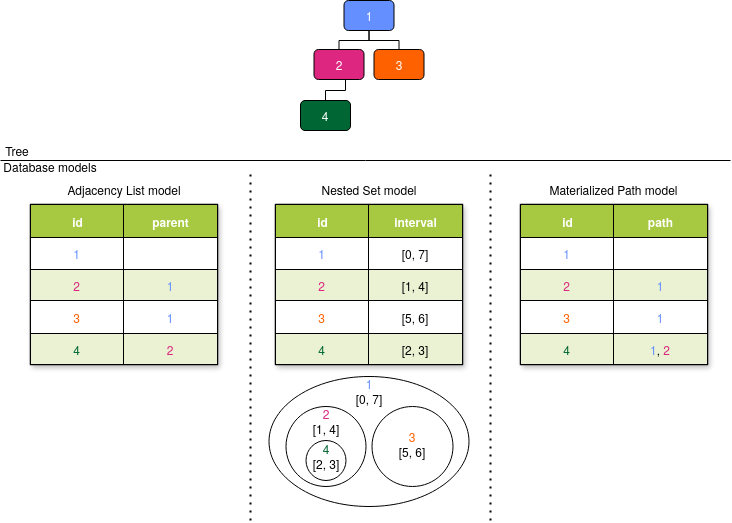
\includegraphics[scale=0.6]{./images/tree-map.drawio.png}
	\caption{Comparison of the Adjacency List, Nested Set, and Materialized Path models.}
\end{figure}

% It is worth noting, that for each of these models, we will have to sepparately delete all
% processes that are stored in the folder
\definecolor{darkgreen}{rgb}{0.0, 0.45, 0.0}
\newcommand{\goodcomplexity}[1]{\vspace{.4em}\textcolor{darkgreen}{\checkmark}\vspace{.4em}}
\newcommand{\mediumcomplexity}[1]{\vspace{.4em}\textcolor{orange}{\textcircled{}}\vspace{.4em}}
\newcommand{\badcomplexity}[1]{\vspace{.4em}\textcolor{red}{X}\vspace{.4em}}

\newcommand{\goodefficency}[1]{\textcolor{darkgreen}{\checkmark}}
\newcommand{\mediumefficency}[1]{\textcolor{orange}{\textcircled{}}}
\newcommand{\badefficency}[1]{\textcolor{red}{X}}

\begin{figure}[H]
	\centering

	\begin{tabular}{ | m{7.45em} | m{7em} | m{7em} | m{7em} | }
		\hline
		                                                               & Adjacency List                                                    & Nested Set              & Materialized Path \\
		\hline
		% ------------------------------------------------------------------------------
		find children                                                  & \goodcomplexity{Easy} \goodefficency{efficient}                   &
		\badcomplexity{Complex} \badefficency{inefficient}             & \goodcomplexity{Easy}
		\mediumefficency{somewhat inefficient}                                                                                                                                           \\
		\hline
		% ------------------------------------------------------------------------------
		find descendants                                               & \goodcomplexity{Easy} \mediumefficency{somewhat inefficient}      &
		\goodcomplexity{Easy} \goodefficency{efficient}                &
		\goodcomplexity{Easy} \goodefficency{efficient}                                                                                                                                  \\
		\hline
		% ------------------------------------------------------------------------------
		find parent                                                    & \goodcomplexity{Easy} \goodefficency{efficient}                   & \badcomplexity{Complex}
		\badefficency{inefficient}                                     & \goodcomplexity{Easy}  \goodefficency{efficient}                                                                \\
		\hline
		% ------------------------------------------------------------------------------
		find ancestors                                                 & \goodcomplexity{Easy} \goodefficency{efficient}                   &
		\goodcomplexity{Easy} \goodefficency{efficient}                & \goodcomplexity{Easy}
		\goodefficency{efficient}                                                                                                                                                        \\
		\hline
		% ------------------------------------------------------------------------------
		add nodes                                                      & \goodcomplexity{Easy} \goodefficency{efficient}                   &
		\badcomplexity{Complex} \mediumefficency{possibly inefficient} & \goodcomplexity{Easy
		and} \goodefficency{efficient}                                                                                                                                                   \\
		\hline
		% ------------------------------------------------------------------------------
		remove nodes                                                   & \goodcomplexity{Easy} \mediumefficency{somewhat inefficient}      &
		\goodcomplexity{Easy} \mediumefficency{possibly inefficient}   &
		\goodcomplexity{Moderately complex} \goodcomplexity{somewhat inefficient}                                                                                                        \\
		\hline
		% ------------------------------------------------------------------------------
		move node                                                      & \goodcomplexity{Easy} \goodcomplexity{efficient}                  & \badcomplexity{Complex}
		\badefficency{inefficient}                                     & \mediumcomplexity{Moderately complex} \badcomplexity{inefficient}                                               \\
		\hline
		% ------------------------------------------------------------------------------
	\end{tabular}

	\vspace{.5em}

	\begin{tabular}{r@{: }l r@{: }l r@{: }l}
		\goodcomplexity{\textcircled{}}\vspace{-.8em} \_ & Easy query                        & \mediumcomplexity{}\vspace{-.8em} \_ &
		Moderately complex query                         & \badcomplexity{}\vspace{-.8em} \_ & Complex query                          \\

		\_ \goodefficency{\textcircled{}}                & Efficient                         & \_ \mediumefficency{}                &
		Moderately efficient                             & \_ \badefficency{}                & Inefficient                            \\
	\end{tabular}


	\caption{Comparison between Adjacency List, Nested Set and Materialized Path models.}
	\label{fig:comparison-db-tree-models}
\end{figure}

To choose the right model, we have to consider the requirements of the MS.
Users need to be able to view, add, delete and remove folders.
It becomes immediately clear, that the Nested Set model is not suitable for the MS, as
adding, removing and moving nodes is inefficient.
% The nested set model appears to be more useful for some analytical workloads.
That leaves us with the adjacency list and materialized path models.
%
The materialized path model has two small advantages: finding descendants and removing a
folder together with its subtree is easier.
Both queries only require a simple string comparison.
%
% The materialized path model has two small advantages, finding descendants is easier as it
% only requires a query with a simple string comparison, and the same goes for removing a
% folder and its subtree. 
%
However, the adjacency list model isn't far behind on those two points, and is
substantially more efficient when it comes to moving nodes.
Furthermore, the adjacency list model is better at finding children, which is more
valuable to the MS than finding descendants, as the Process view will only show the
children.
For those reasons, the MS will use the adjacency list model to store the folder structure.

\subsection{Storing Assets Inside Folders}

Once the folder structure is implemented, it still is necessary to store assets inside
folders.
This thesis only implemented this feature for processes
\ref{cha:relatedwork:proceed-assets}, however, the same principle could be applied to
other assets.
A complete redesign of the process' data structures isn't feasible, as it would require
rewriting a large part of the MS.
For this reason a simple expansion to the data structure was chosen, where analogous to
the adjacency list model, each process stores a reference to the folder it is stored in.
This way, when moving a folder, it isn't required to update anything other than the
folder.
Moving an asset to another folder only requires updating the asset's reference.

% Folders are nodes in a rooted tree structure with a name and a description.
% Folders can contain other folders and assets.

% Each environment will have a folder structure to store its processes.
% The root folder is created when the environment is created.
% Each root folder and all of its children are contained by one and only one environment \ref{cha:conceptanddesign:environments}.


% Since the root folder belongs to only one environment, and all folders are stored below
% one root folder, all folders belong to only one environment.
% Processes will then store a reference to the folder they're stored in.

% TODO: ask kai if I should explain rooted trees - would be nice to cookup a formal def


\section{Environments}
\label{cha:conceptanddesign:environments}

Conceptually, environments are where everything except users are stored.
Users aren't stored in environments as they can be a part of multiple environments.
Instead, the MS stores memberships, which specify that a user is part of an environment.

There are two types of environments, personal and organization environments.
Personal environments are intended for personal use and organization environments are intended
for organizations.

\subsection{Personal Environments}
\label{cha:conceptanddesign:environments:personal}

Personal environments are assigned to each user once they sign in.
%NOTE: remove the part with owner
The user for which the environment is created is the only member of this
environment, and is therefore called the owner.
No other users be a part of this environment.
%TODO: forward ref to folders
Personal environment only allow users to create and manage processes and folders,
while other features offered by the MS can only be used in organization environments
\ref{cha:conceptanddesign:environments:organization}.

\subsection{Organization Environments}
\label{cha:conceptanddesign:environments:organization}

Organization environments are intended to be used by organizations, thus they can have a
name, description and a logo.
In contrast to personal environments, users are allowed to use all the MS' features in
an organization environment.

% They extend the feature set of personal environments, the enabled
% resources \ref{cha:relatedwork:proceedroles:ms-resources-actions} for organization
% environments can be determined when deploying a MS instance.

Organization environments can also have multiple Users that are part of it, these are
called members.

\subsection{Environment Memberships}
\label{cha:conceptanddesign:environments:memberships}
% TODO: maybe merge this with the role stuff
% to do that however, roles would have to be added to the environment section, and I dont
% know if that's the right choice as it is a big topic

To keep track of which users are part of an environment, a new management asset will be
added: memberships.
Each membership links one user to one environment, specifying that the user is part of
that environment.

\subsection{Storing Assets inside Environments}
\label{cha:conceptanddesign:environments:storing-assets}

All assets within the MS \ref{cha:relatedwork:proceed-assets}, including folders,
will be modified, so that each asset instance establishes a clear association with a single environment.
Every asset will store a reference to the environment it belongs to.
This reference is immutable, with the only exception being when assets are transferred
from a guest user to an authenticated user \ref{cha:conceptanddesign:users:mergeguestuser}.

Processes and folders will be contained within folders, which implies that they belong to
the same environment as their root folder.
This means that for these assets, we are storing the environment they belong to twice.
Storing redundant information is risky as it can lead to inconsistencies if updates aren't
done correctly.
For instance if a folder's environment reference is changed, but those of its children
are not, then the folder structure would span across two environments.
This risk is mitigated by the fact, that the environment reference of assets is immutable.

% The key principle is that every asset belongs to one and only one environment, and this
% association can be easily identified.

% All of the MS' assets will only change in one way, they will somehow linked to an
% environment and only one.
% For processes, they're contained in a folder, such that they clearly belong to one
% environment. for other assets, they will store a reference to the environment they belong
% to.
% The important part is that each asset belongs to exactly one environment, and this
% environment can be identified.



\subsection{Environment Selection}
% TODO: maybe back this up with some research, although this isn't that kind of thesis

Users will be a part of multiple environments, and they will need to be able to work on
all of them.
There are two ways of accomplishing this: the user can select one environment at a time,
or he can work on multiple environments at the same time.
%
% As environments contain many features, it isn't feasible to show all of them at the same
% time, as this would clutter the interface, some level of selection is necessary.
%
Environments contain many features and views, making it unfeasible to show them all
simultaneously for many environments.
Thus, some level of selection is necessary to avoid cluttering the interface.

%
This selection could be granular, where the user selects per view which environment he
wants to work on, however this could lead to confusion, if the user switches views and
forgets that he's working on a different environment.
For this reason, we chose to have a global environment selection, i.e. all the elements in
the UI will show the assets and views of the selected environment.

There are two methods of accomplishing environment selection: implicit and explicit.
In the implicit method, the selected environment is managed internally and is not
reflected to the user in the URL, this could be accomplished by storing the selected
environment in the user's cookies or in the browser's local storage for example.
In the explicit method, the environment is encoded in the URL,
making the current environment clearly visible.
Of course a combination of both methods is also possible, but in order to keep the
implementation simple, we only chose one.
The implicit method has the advantage that the URLs are shorter and easier to read,
however it has the disadvantage, that some links can't be shared, since the implicitly
selected environment of another user might not be the same.
For this reason, the explicit method was chosen as it allows users to share links with the
cost of longer URLs.

\section{Roles}
\label{cha:conceptanddesign:roles}

% Roles are used to determine what a user can do with an asset. 
% Before the implementation of this thesis, roles in the MS
% \ref{cha:relatedwork:proceedroles} were global,
% meaning that their permissions applied to all assets in the MS.
% With the introduction of environments and the folder structure, this no longer makes sense.
% Roles will be modified to be associated with one organization environment, and they will only apply to
% the assets in that organization environment.
% In personal environments, there is only one user, and he can perform all actions on all of
% his assets.
Roles define what actions a user can perform on an asset. Prior to the changes introduced
in this thesis, roles in MS \ref{cha:relatedwork:proceedroles} were global,
meaning their permissions applied universally
to all assets across the system.
However, with the addition of environments and a folder structure, this approach is no longer practical.
Roles will now be tied to a specific organization environment,
restricting their permissions to assets within that particular environment.
In personal environments, where there is only one user, the user will have
full control and be able to perform all actions on his assets without restriction.

Folders allow organizations to mirror their hierarchical structure, but this wouldn't be
entirely useful if roles applied to all assets inside the environment.
For this reason, roles can now be associated to a folder.
%
A role can define permissions for many assets, of which not all can be stored in folders.
If a role is associated with a folder, then, only the permissions that are for assets that
can be stored in folders, will be affected by the association.
% The permissions of the role that apply to assets that can be stored in folders, 
% will only apply to the assets that are in the folder's subtree.
%
The permissions of roles that are associated with a folder cascade down the
folder structure, i.e. a role associated to a folder will also apply to all of its
descendants.
In this thesis, the folder structure was only implemented for processes,
this means that only the permissions for processes and folders will apply to the
associated folder's descendants.
Roles that aren't associated to a folder will continue to apply to all assets in the environment.
% As roles are meant to mirror a users position in an organization, they're only available
% for organization environments.

\begin{figure}[H]
	\centering
	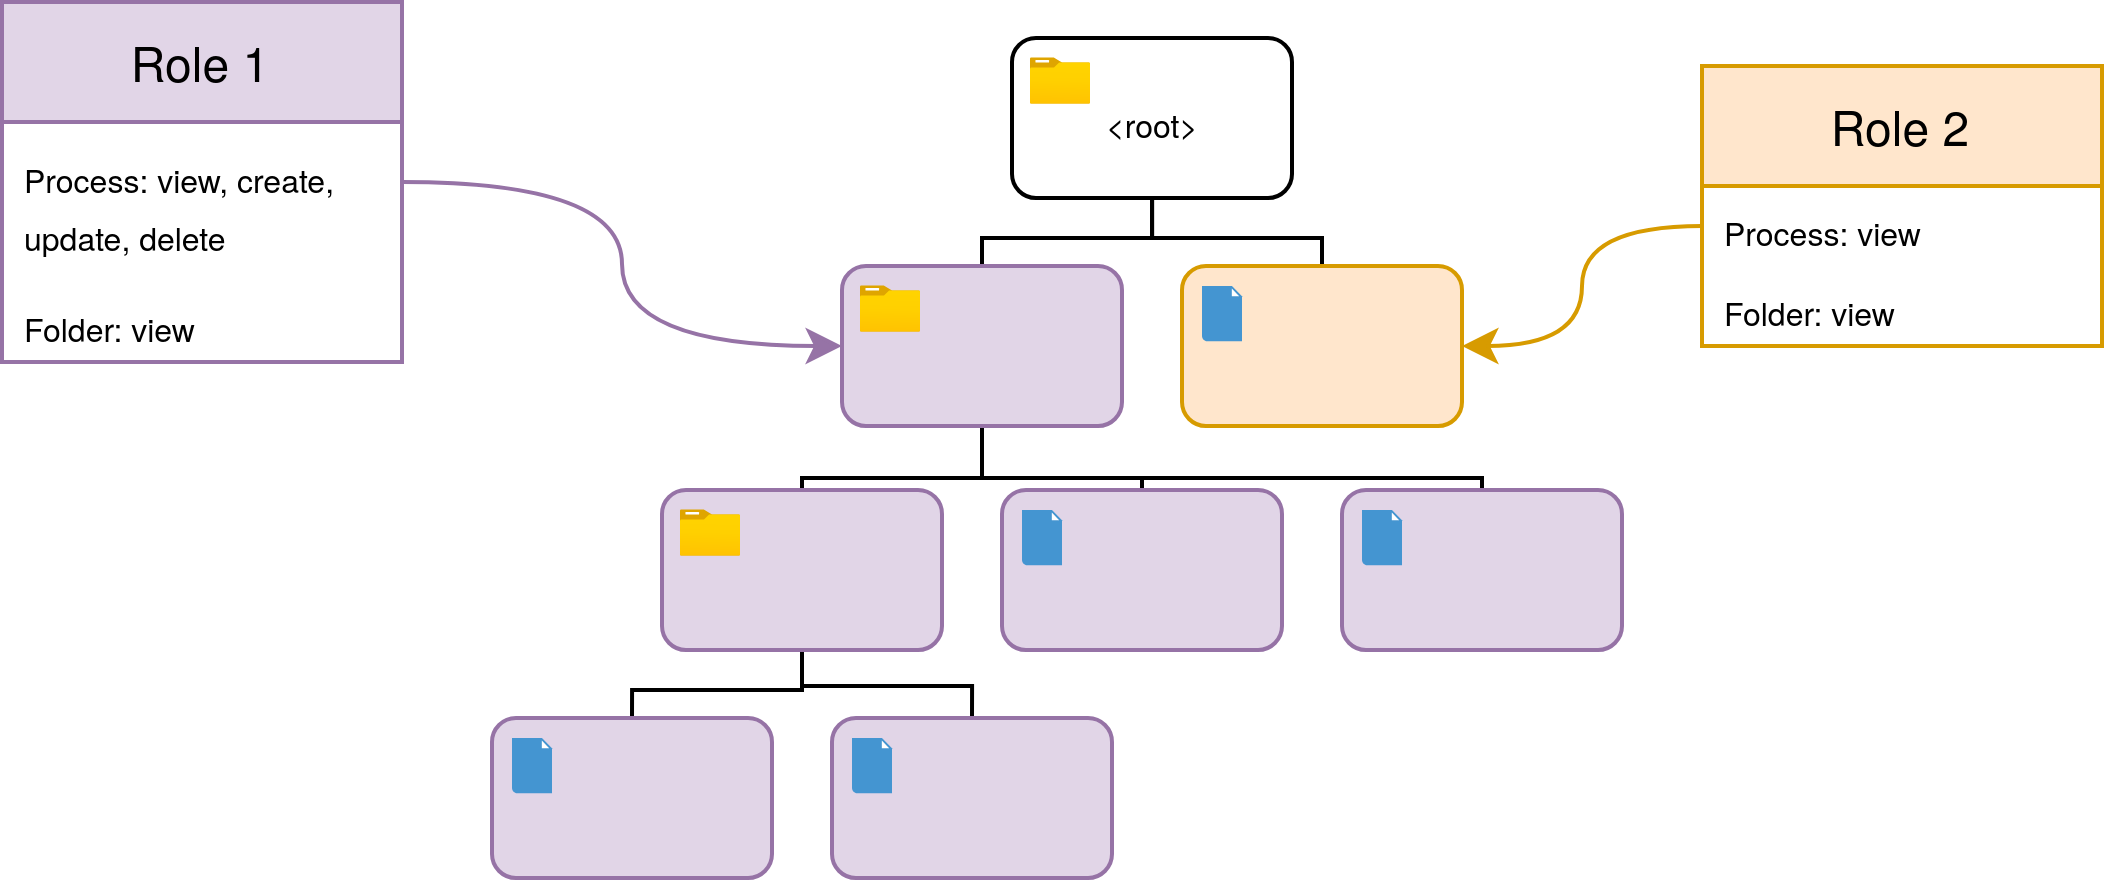
\includegraphics[scale=0.2]{./images/tree-roles.drawio.png}
	\caption{Permissions of roles cascade down the folder structure.}
\end{figure}

If a user's role allows him to view assets and is associated to a folder, then the user
also has the permission to view all ancestors of the folder.
But this permission is only restricted to the parent folders, not the contents of the parent folders.
This allows users to navigate the folder structure until they reach the assets they're
allowed to view and manage.

% TODOFIG: show how user can view path to his folder

\subsection{New Resources}

% TODO: mention that each role comes with an action
With the introduction of environments, all the previously available resources still hold
the same meaning, with the difference that they are now associated with an environment.
Additionally, two new Resources where introduced, for which roles can specify permissions:

\begin{itemize}
	\item \textbf{Folder}: Folders are used to organize assets in an environment.
	      If a role is associated to a folder, then the permissions for the folder apply to that
	      folder and all folders
	      \begin{itemize}
		      \item \lstinline{view}: Allows the user to view the folder, its name and description.
		            This doesn't necessarily mean that the user can view the assets inside the folder,
		            as he still needs the \lstinline{view} permission for each children, which would be
		            the case, if the role is associated to a folder.
		      \item \lstinline{create}: The user can create new folders inside the folder he has this
		            permission for.
		      \item \lstinline{update}: The user can update the folder's name and description, as
		            well as move the folder, to another folder where he has the \lstinline{create}
		            permission.

		            % TODO: deleting a folder deletes the processes inside of it
		            % maybe this needs to be checked
		      \item \lstinline{delete}: The user can delete the folder.
	      \end{itemize}
	\item \textbf{Environment}: Folders are used to organize assets in an environment.
	      \begin{itemize}
		      % TODO: members cannot actually see the environments name and description 
		      \item \lstinline{view}, \lstinline{create}: These actions are not implemented for
		            environments.
		            Each member can view the name and description of the environment.
		            \lstinline{create} can't exist as it implies that the environment doesn't exist
		            yet, and therefore a role that contains it cannot exist.
		      \item \lstinline{update}: The user can update the environment's name, description
		            and contact number.
		      \item \lstinline{delete}: Allows the user to delete the environment with all its
		            assets, this is only possible for organization environments,
	      \end{itemize}
\end{itemize}

\subsection{Enforcing Permissions Based on Folder Structure}

In order to enforce permissions based on the folder structure, it is necessary to fetch
the newest state of the folder structure every time a user wants to perform an action on an asset.
Roles can't store a representation of the folder structure, as it might become outdated.
Since permissions need to be verified, for many requests in the MS, and also in the user's browser, to
adapt the UI, we decided to compute and cache a representation of the folder structure of
every organization environment, from which an asset is requested.
This representation is also sent to the user's browser.

% TODO: roles send folder structure to user, is this bad? how could we mitigate it

\subsection{Default Roles}

For each organization environment two roles will be created, which cannot be deleted and
cannot be associated to a folder:

\begin{itemize}
	\item \lstinline{@admin}: This role has all permissions for all assets in the
	      organization environment and it is first assigned to the user that creates the organization environment.
	      Only users with the \lstinline{@admin} role can add new users to this role.
	\item \lstinline{@everyone}: The permissions in this role apply to for all the users
	      that are part of the organization environment. The permissions in this role start out
	      empty, but can be modified.
\end{itemize}
